\documentclass[12pt,a4paper]{article}
\usepackage[utf8]{inputenc}
\usepackage[T1]{fontenc}
\usepackage[french]{babel}
\usepackage{amsmath, amssymb, amsfonts}
\usepackage{graphicx}
\usepackage{geometry}
\usepackage{hyperref}
\usepackage{fancyhdr}
\usepackage{setspace}
\usepackage{lmodern}
\usepackage{csquotes}
\usepackage[most]{tcolorbox}

\geometry{margin=2.5cm}
\pagestyle{fancy}
\fancyhf{}
\rhead{\thepage}
\lhead{Théorie de la spéculation – thèse de Louis Bachelier, 1900}

\usepackage{titling}
\renewcommand\maketitlehooka{\null\mbox{}\vfill}
\renewcommand\maketitlehookd{\vfill\null}

\title{\Huge{\textbf{Théorie de la spéculation\\ Louis Bachelier, 1900}}\\ \medskip
      \Huge{\textit{Article résumé}}\vspace*{0.7cm}}
\author{\LARGE{Alexis VO}\vspace{1cm}\\ \medskip
      Université Paris-Saclay\\École polytechnique}
\date{\vspace{0.2cm}\today}

% === BEGIN DOCUMENT ===
\begin{document}

\vspace{\fill}
  \maketitle
\vspace{\fill}

\newpage

\tableofcontents

\begin{abstract}
En 1900, Louis Bachelier soutient une thèse qui donnera par la suite les bases d’une approche probabiliste des marchés financiers : \textit{La théorie de la spéculation}. Je vous propose dans cet article un résumé après une lecture approfondie de ce texte fondateur. Il s'inscrit dans le cadre de mon stage ayant pour sujet principal le \textit{Modèle de Cox Ross Rubinstein}. Nous évoquerons les idées de ce mathématicien novateur dans leur contexte historique, en analysant ses modèles mathématiques, et en mettant en lumière leur influence sur la finance moderne. Enfin, nous présenterons les concepts de cours vrai, de prime, d’option et d’équation de la diffusion à travers la modélisation proposée par Bachelier.
\end{abstract}

\newpage

\section{Introduction générale}

\subsection{Contexte historique}

Au tournant du XX\textsuperscript{e} siècle, les marchés financiers comme la \textit{Bourse de Paris}, connaissent une forte expansion. Les opérations de spéculation y sont nombreuses, mais leur analyse reste essentiellement empirique et intuitive. À cette époque, la probabilité est encore principalement appliquée aux jeux de hasard. Nul ne l'imagine l’appliquer aux mouvements financiers, considérés encore comme trop chaotiques.

C’est dans ce contexte que Louis Bachelier, jeune mathématicien français, propose en 1900 une thèse intitulée \textit{Théorie de la spéculation}. Il modélise mathématiquement les fluctuations boursières en utilisant le calcul des probabilités. Il devient alors le fondateur des mathématiques financières.

\subsection{Présentation de Louis Bachelier}

Louis Bachelier (1870–1946) est un mathématicien français formé à la Sorbonne. Sa thèse est novatrice à bien des égards : elle est la première à proposer une modélisation stochastique du marché financier. Bien qu’initialement peu reconnue, son œuvre sera redécouverte au XX\textsuperscript{e} siècle, notamment par les économistes et mathématiciens anglo-saxons.

Il est aujourd’hui considéré comme un précurseur de la finance quantitative et un pionnier du mouvement brownien en mathématiques.

\subsection{Objectifs de l'article}

Je vous propore dans le présent article un résumé d'une lecture active de la thèse de Bachelier (66 pages). Il vise tout d'abord à présenter les idées clés de la \textit{Théorie de la spéculation} dans un langage accessible aux étudiants de licence. Nous y expliquerons notamment les modèles mathématiques introduits (cours vrai, loi de probabilité, diffusion, etc.) et nous conclurons par les liens entre les intuitions de Bachelier et les développements ultérieurs en finance moderne.

% \subsection{Principales contributions de la thèse}

% Dans sa thèse, Bachelier introduit plusieurs concepts fondamentaux. Il modélise dans un premier temps les variations de cours comme un phénomène aléatoire, posant les bases du mouvement brownien avant même Einstein (qui publie un article sur ce sujet en 1905) ! Il établit ensuite une loi de probabilité pour les fluctuations de marché, inspirée de la loi normale de Gauss. D'autre part, il formalise des notions toujours utilisées aujourd’hui comme le cours « vrai », les primes, et les options. Enfin, il énonce que dans un marché équilibré, l’espérance mathématique du spéculateur est nulle, anticipant ainsi le très important \textit{principe d’absence d’arbitrage}.

% Ces apports font de sa thèse un texte visionnaire, fondateur de la finance moderne, bien avant l’avènement de modèles comme celui de Black-Scholes par exemple.

\section{La Bourse et ses mécanismes au XIX\textsuperscript{e} siècle}

\subsection{Les opérations de Bourse}

Dans les premières pages de sa thèse, Bachelier commence par rappeler les différents types d'opérations que l’on rencontre à la Bourse de Paris, structurées principalement autour des \textit{opérations à terme} :

\begin{itemize}
  \item Les \textit{opérations fermes} : engagements irrévocables d'achat ou de vente à une date future ;
  \item Les \textit{opérations à prime} : options donnant le droit, mais non l'obligation, d’acheter ou de vendre.
\end{itemize}

Il note que ces opérations peuvent se combiner de manière très variée, notamment dans le cas de primes multiples. Cette structuration montre que le marché de l’époque n’est pas seulement un lieu de transaction comptant i.e. un lieu où le réglement ne s'effectue pas seulement à l'achat, mais aussi un lieu de spéculation sur l’évolution future des cours.

\subsection{Opérations fermes et opérations à prime}

Les opérations fermes s’apparentent à des ventes classiques, mais décalées dans le temps. À la liquidation -- qui a lieu en fin de mois -- seule la différence de cours est réglée. Le \textit{cours de compensation} est alors utilisé pour solder les positions. Par exemple, un achat ferme donne un gain si le prix de vente est supérieur au prix d’achat, et une perte dans le cas contraire.

Quant aux opérations à prime, elles ressemblent aux options actuelles :
\begin{itemize}
  \item L’acheteur de la prime paie un montant fixe (la prime) pour bénéficier d’un gain potentiel en cas de hausse (prime à la hausse) ou de baisse (prime à la baisse).
  \item Sa perte est limitée à la prime versée, tandis que son gain est théoriquement illimité.
  \item Le vendeur de prime, à l’inverse, perçoit une prime fixe mais s’expose à une perte potentielle importante.
\end{itemize}
C'est typiquement ce que l'on appelle aujourd'hui les options d'achat et de vente (call/put).\\
Bachelier illustre ces opérations par des représentations géométriques (p.~25–26), où l'on peut observer les bénéfices en fonction des cours. Nous étudierons cela dans une autre section.

\subsection{Reports, coupons et cours de compensation}

Le \textit{report} est une opération financière qui permet à un acheteur à terme de prolonger sa position au mois suivant. Il paie alors un intérêt au vendeur, sauf cas exceptionnel où cet intérêt est négatif, appelé \textit{déport}.

Sur les valeurs à revenu fixe comme la rente 3~\% de l’époque, les acheteurs perçoivent des \textit{coupons trimestriels}, ce qui crée une asymétrie. D'une part l’acheteur touche les coupons mais paie le report. D'autre part, le vendeur touche le report mais doit verser les coupons.

Bachelier note que cette situation peut générer un avantage pour certaines positions à long terme, comme les \textit{rentes reportables}, où l’achat et le report prolongé sont utilisés pour capter le rendement du coupon.

Le \textit{cours de compensation} est le prix de référence utilisé lors de la liquidation pour évaluer les gains ou pertes. Il est crucial dans la détermination des résultats des opérations à terme.

\subsection{Cours vrai et cours équivalent}

Dans sa \emph{Théorie de la spéculation} (1900), Louis Bachelier introduit la notion de \textbf{cours vrai}, qu’il définit comme le prix \textbf{idéal} d’un actif à un instant donné, tenant compte de l’ensemble des informations disponibles et de toutes les probabilités futures d’évolution du cours.

\begin{quote}
    \emph{« Le cours vrai est celui qui serait obtenu s’il était possible de prendre en considération toutes les causes d’ordre économique ou politique susceptibles d’influer sur le marché, ainsi que toutes les chances d’accroissement ou de diminution des valeurs. »} \\
    — Louis Bachelier, \emph{Théorie de la spéculation}, p. 18
\end{quote}

Cette notion est essentielle. Selon lui, le cours coté sur le marché n’est pas nécessairement le plus juste. Il propose de corriger ce cours en tenant compte des intérêts liés aux coupons à venir, des effets du report, et de la date de liquidation. Autrement dit, le cours vrai est un idéal probabiliste, inaccessible mais vers lequel tend la spéculation rationnelle. Il peut être interprété comme l’\textit{espérance mathématique} du prix futur de l’actif, selon les probabilités anticipées par les spéculateurs. Il est en général \textit{inobservable}, mais sert de référence théorique autour de laquelle fluctue le cours réel.

Il définit alors des \textit{cours équivalents} comme des prix futurs attendus, ajustés pour refléter la position dans le mois.

La \textit{courbe des cours vrais} est présentée comme une fonction linéaire entre deux liquidations. Cette courbe est centrale pour déterminer la \textit{valeur actualisée} des positions.

Enfin, le mathématicien insiste sur l'importance de cette correction car elle permet de calculer des espérances mathématiques équitables. C'est la base de son raisonnement probabiliste.

\subsection{Illustrons cela par un exemple}

Soit une action valant aujourd’hui 100~€. On estime qu’il y a :
\begin{itemize}
  \item 50\,\% de chances qu’elle monte à 110~€,
  \item 50\,\% de chances qu’elle descende à 90~€.
\end{itemize}

On calcule alors le cours vrai comme la moyenne pondérée :
\[
\text{Cours vrai} = 0{,}5 \times 110 + 0{,}5 \times 90 = 100~euros
\]

Dans cet exemple, le cours observé coïncide avec le cours vrai, traduisant une situation d’\textit{équilibre spéculatif}.

Ce concept est fondamental, car il relie le \textit{prix d’un actif} à son \textit{comportement probabiliste} anticipé, amorçant ainsi les bases de la modélisation financière moderne.

\bigskip

\noindent
Au terme de cette première partie, nous avons  posé les bases de la thèse de Bachelier. Un marché organisé autour d’opérations structurées, une dynamique temporelle claire, et l’introduction d'un point de vue mathématique du comportement des cours. Dans la suite, Bachelier utilise ces outils pour bâtir un modèle probabiliste rigoureux de la spéculation.

\section{Modélisation mathématique des opérations}

\subsection{Achat, vente et prime}

Comme évoqué précédemment, les \textit{primes} sont l’ancêtre direct des options. Elles sont modélisées comme une combinaison asymétrique d’exposition au risque. L’\textit{achat à prime} donne un bénéfice croissant au-delà d’un certain seuil i.e. le \textit{pied de la prime}, mais limite la perte à la prime versée. La représentation graphique est une droite horizontale (perte fixe) en dessous du seuil, et une pente $+1$ au-dessus.

La figure proposée par Bachelier (fig.~4, p.~30) illustre cela : une \textit{ligne brisée} dont le point de rupture correspond au seuil de rentabilité.

\begin{center}
  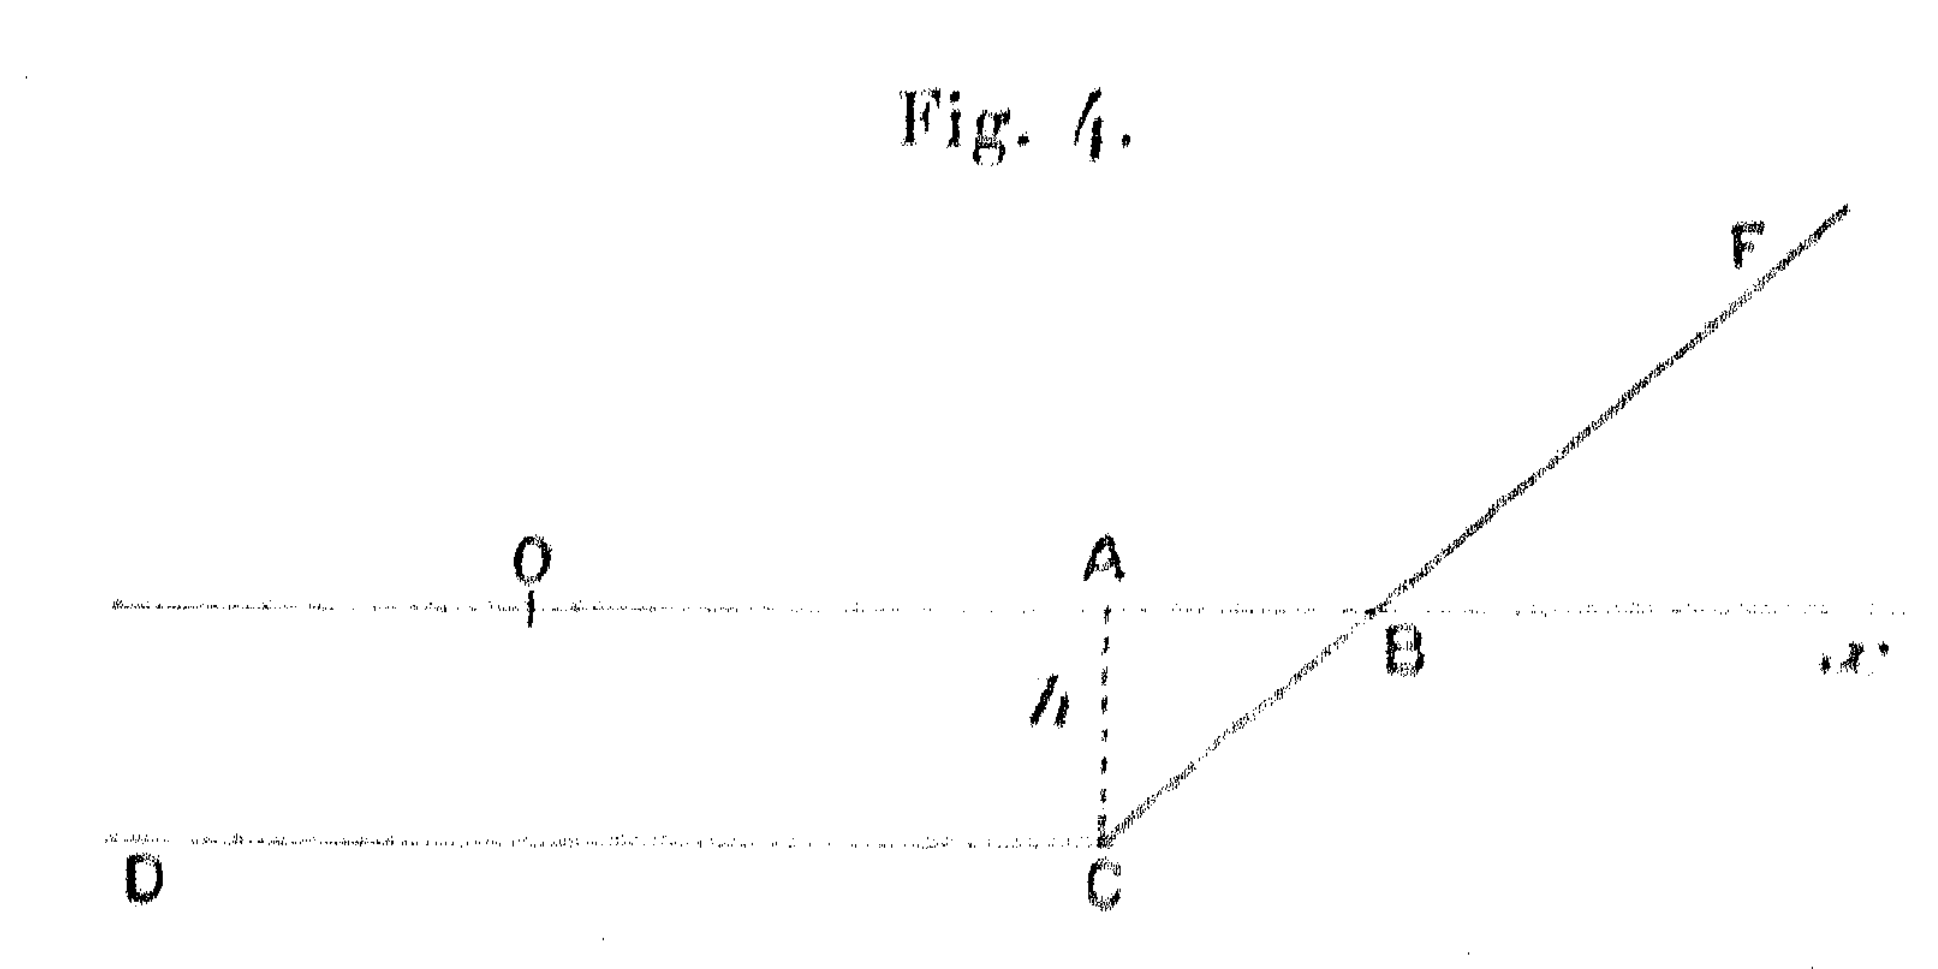
\includegraphics[width=0.5\textwidth]{fig4.png}
\end{center}

Inversement, une \textit{vente à prime} est représentée par une droite brisée en pente négative au-delà du seuil, et plate (gain constant) en dessous. Le vendeur gagne la prime si le marché ne dépasse pas un certain niveau, mais perd au-delà.

Bachelier insiste sur le fait que les marchés à prime permettent de \textit{limiter les pertes}, ce qui les rend attractifs pour certains spéculateurs. Mais cela a un coût ! L'espérance mathématique de la prime est construite de manière à maintenir une neutralité statistique. Il revient sur ce principe plus loin dans sa thèse.

\subsection{Options et stellage}

\begin{quote}
    \emph{« Il est même possible de spéculer uniquement sur la variation absolue du cours, sans égard à la direction dans laquelle elle se produit. »} \\
    — Louis Bachelier, \emph{Théorie de la spéculation}, p. 50
\end{quote}

En complément des opérations simples, le mathématicien introduit (p.~31) ce qu’il appelle des \textit{options} (au sens moderne du terme), c’est-à-dire des instruments hybrides entre le ferme et la prime. En fait, aujourd'hui cela revient à acheter simultanément une option d'achat (call) de prix d'exercice $K$ (le strike), et une option de vente (put) de même strike et même maturity.

Il donne l’exemple d’une \textit{option du double} : une position qui donne droit à deux unités de gain en cas de hausse, mais seulement à une unité de perte en cas de baisse. On parle aujourd’hui d’option asymétrique. De telles structures permettent de moduler le profil de risque selon les anticipations.

De plus, il décrit le \textit{stellage} -- ou \textit{double prime} -- constitué d’une prime à la hausse combinée avec une prime à la baisse. On l’interprète aujourd’hui comme une \textit{stratégie de tunnel, appelée straddle}.

Ce montage donne :
\begin{itemize}
  \item un gain si le cours s’éloigne significativement du cours d’exercice i.e. volatilité grande,
  \item une perte limitée à la somme des deux primes si le cours reste stable.
\end{itemize}

Le stellage est donc une \textit{stratégie directionnellement neutre}, qui mise uniquement sur l’ampleur des variations du cours, et non pas sur la direction du marché.

\begin{center}
    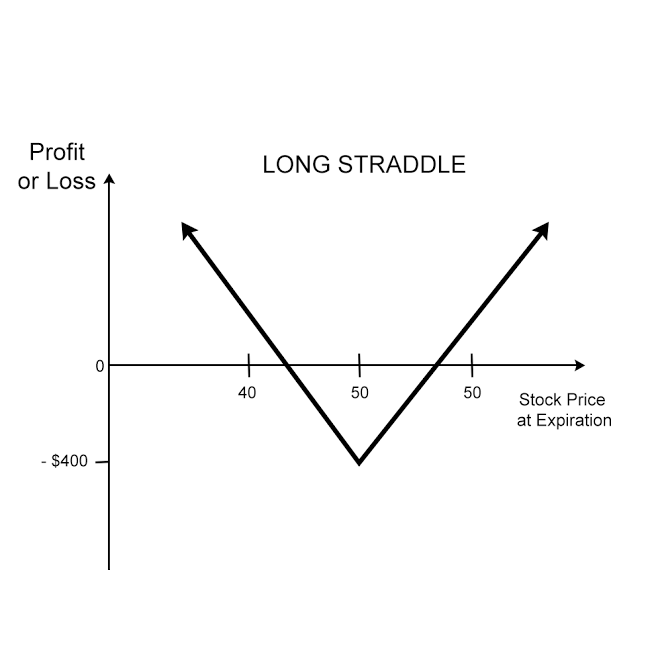
\includegraphics[width=0.4\textwidth]{strad.png}
\end{center}

\medskip

\subsection{Illustrons cela par un exemple}

\begin{itemize}
    \item Prix actuel de l’action : 100~€ ;
    \item Prix d’exercice : $K = 100$~€ ;
    \item Le spéculateur achète :
    \begin{itemize}
        \item un call 100 pour 5~€,
        \item un put 100 pour 5~€.
    \end{itemize}
    \item \textbf{Coût total du straddle} : 10~€.
\end{itemize}

\begin{center}
\begin{tabular}{|c|c|c|c|c|}
\hline
\textbf{Cours à l’échéance} & \textbf{Gain call} & \textbf{Gain put} & \textbf{Gain total} & \textbf{Bénéfice net} \\
\hline
100~€ & 0 & 0 & 0 & \textcolor{red}{--10~€} \\
\hline
110~€ & 10 & 0 & 10 & 0~€ \\
\hline
120~€ & 20 & 0 & 20 & \textcolor{green!60!black}{+10~€} \\
\hline
90~€ & 0 & 10 & 10 & 0~€ \\
\hline
80~€ & 0 & 20 & 20 & \textcolor{green!60!black}{+10~€} \\
\hline
\end{tabular}
\end{center}

Il s’agit d’un pari sur une forte \textit{amplitude des fluctuations} à venir. Dans le modèle de Bachelier, où les variations de prix sont modélisées par un mouvement brownien, le straddle a une valeur croissante avec la \textit{dispersion attendue} des prix, c’est-à-dire leur \textit{variance}. Ce raisonnement annonce les méthodes modernes de valorisation d’options basées sur la \textit{volatilité implicite}.


\bigskip

\noindent
Au terme de cette seconde partie, nous avons compris que cette modélisation des opérations financières est l’un des apports majeurs de Bachelier dans les mathématiques financières que nous connaissons aujourd'hui. Elle permet de visualiser les profils de gains et pertes associés à chaque type d’opération, et prépare le terrain à une analyse probabiliste des stratégies, développée dans les sections suivantes.

\section{Probabilités dans les opérations financières}

\subsection{Probabilités mathématiques et spéculatives}

Le mathématicien précurseur distingue deux types de probabilités dans le contexte des opérations financières :

\begin{itemize}
    \item Les \textit{probabilités mathématiques} sont déterminées \textit{a priori}, sur la base d’hypothèses de symétrie ou de lois connues. Elles sont typiques des jeux de hasard et permettent une modélisation probabiliste rigoureuse.

    \item Les \textit{probabilités spéculatives}, quant à elles, traduisent les anticipations subjectives des agents économiques sur l’évolution future des cours. Ces probabilités sont liées à des jugements personnels basés sur des facteurs économiques, politiques ou psychologiques.
\end{itemize}

Bien que les variations des cours soient imprévisibles, on peut à un instant donné leur associer une \textit{loi de probabilité} décrivant l’état statistique du marché. Dans sa thèse, Bachelier postule que le marché dans son ensemble est \textit{neutre} : il n’anticipe ni la hausse ni la baisse. Cela se traduit mathématiquement par la symétrie de la loi de probabilité autour d’un \textit{cours vrai}.

La fonction de densité de probabilité \( p(x) \) représente la probabilité que le cours relatif, c’est-à-dire l’écart entre le cours effectif et le cours vrai, soit égal à \( x \). Cette densité est symétrique autour de zéro, ce qui s’exprime par :

\[
p(x) = p(-x) \quad \text{pour tout } x \in \mathbb{R}.
\]

Cette propriété, dite de \textit{symétrie ou parité}, traduit l’idée que les fluctuations positives et négatives de même amplitude sont équiprobables, en l’absence de biais directionnel. Elle correspond à un marché \textit{neutre}, où aucune tendance ascendante ou descendante ne domine. On retrouve ici une hypothèse d’\textit{absence d’information privilégiée}, qui anticipe l’idée moderne de \emph{marche aléatoire sans drift}.

On verra dans la section suivante que cette loi est modélisée par une densité normale centrée, solution de l'équation de la chaleur.\\

\subsection{Espérance mathématique et équité du marché}

L’espérance mathématique joue un rôle fondamental dans l’évaluation des jeux de hasard et des opérations financières. Elle est définie comme le produit du gain possible par la probabilité de ce gain. Un jeu est dit \textit{équitable} lorsque son espérance est nulle.

\begin{center}
    \og L’espérance mathématique du spéculateur est nulle. \fg\ p. 34
\end{center}

Ce principe de neutralité permet de garantir que, selon la loi de probabilité admise par le marché à un instant donné, aucune opération n’offre un avantage certain. Ainsi, même une stratégie conditionnelle -- par exemple, vendre dès que le cours dépasse un certain seuil -- a une espérance nulle au regard du marché.

L’hypothèse d’espérance nulle traduit une vision idéale du marché : en l’absence d’information privilégiée, chaque spéculation est un \emph{jeu équitable}, sans avantage structurel. Cette condition se traduit par :

\[
\mathbb{E}[X] = \int_{-\infty}^{+\infty} x \, p(x) \, dx = 0.
\]

Cela signifie que, sur le long terme, le spéculateur ne peut espérer ni gain ni perte en moyenne. Ce principe de neutralité garantit qu’aucune opération, même conditionnelle, ne procure d’avantage certain.

\subsection{Illustrons cela par un exemple}

Considérons un actif valant 100~€ à l’instant initial. Un spéculateur s’attend à ce qu’à l’instant $t = 1$, le cours fluctue autour de cette valeur selon la loi de probabilité simplifiée suivante :

\begin{center}
\begin{tabular}{|c|c|}
\hline
\textbf{Écart $x$ au cours vrai} & \textbf{Probabilité $p(x)$} \\
\hline
$-10$ & $0{,}25$ \\
\hline
$0$   & $0{,}50$ \\
\hline
$+10$ & $0{,}25$ \\
\hline
\end{tabular}
\end{center}

Cette loi est clairement \textit{symétrique} autour de $x=0$ : on a $p(x) = p(-x)$.

Espérance mathématique du gain :
\[
\mathbb{E}[x] = (-10) \cdot 0{,}25 + 0 \cdot 0{,}5 + 10 \cdot 0{,}25 = -2{,}5 + 0 + 2{,}5 = 0
\]

L’espérance est donc nulle : le jeu est \textit{équitable}.

\medskip

Même si le spéculateur élabore une stratégie conditionnelle, par exemple vendre dès que le cours dépasse 110~€, ou acheter en dessous de 90~€, la symétrie des probabilités implique que son \emph{gain espéré reste nul}.
Cela formalise l’idée que \textit{le marché, en l’absence d’information asymétrique}, est un système \textit{neutre et équitable} — tout avantage anticipé est compensé, en moyenne, par un désavantage équivalent.

\medskip

Ce formalisme permet de passer d’un raisonnement spéculatif subjectif à une modélisation mathématique des fluctuations boursières. Même si chaque agent agit sur la base de croyances individuelles, le comportement global du marché peut être décrit par une loi de probabilité objective et continue.

\medskip

\noindent
\textbf{Longue remarque : } il peut sembler paradoxal, voire absurde, de modéliser par des outils mathématiques ce qui relève des croyances subjectives de chaque agent économique. En effet, chaque spéculateur agit en fonction d'informations incomplètes, de jugements personnels et d’intuitions, si bien que prévoir l’avenir des cours semble hors de portée du calcul. C'est aussi une réflexion que je me suis faite. Cependant, la puissance de ces outils mathématiques ne réside pas dans la prédiction d’un cours futur déterminé, mais dans la description statistique du \textit{comportement global} du marché. De la même manière qu'en physique statistique on modélise l’agitation thermique de milliards de particules sans connaître leurs trajectoires individuelles, on peut modéliser l'ensemble des anticipations des agents comme un phénomène aléatoire régulier. On utilise d'ailleurs une équation venant de la physique, celle de la chaleur ! Cette régularité émerge lorsque l’on considère non pas un agent isolé, mais une population d’agents ayant des opinions divergentes qui s’équilibrent en moyenne. C’est ce principe qui justifie l’usage d’une densité de probabilité centrée sur un cours ``neutre'' (le cours vrai), et qui donne sens à une approche probabiliste des marchés.

\subsection{Avantage mathématique}

La situation d’un marché parfaitement équitable, où l’espérance mathématique des spéculateurs est nulle, constitue un cas idéal. Cependant, tous les jeux ou opérations financières ne présentent pas cette symétrie parfaite. En pratique, certaines stratégies offrent une probabilité de gain plus élevée que d’autres, ou bien un gain potentiel supérieur à la perte encourue, sans que l’espérance totale ne soit nécessairement nulle.

\medskip

C’est pourquoi Bachelier introduit une notion complémentaire : celle d’\textit{avantage mathématique}, qui permet de quantifier l'asymétrie d'un jeu (la tendance favorable ou défavorable d’un jeu), même lorsqu’il n’est pas strictement équitable.

\medskip

Le mathématicien définit cet avantage comme le rapport entre l’espérance positive et la somme des espérances positive et négative :
\[
\text{Avantage mathématique} = \frac{\text{espérance positive}}{\text{espérance positive} + \text{espérance négative}}
\]

Cette notion complète celle d’espérance mathématique en évaluant l’asymétrie du jeu : un jeu équitable a un avantage de 1/2, tandis qu’un jeu déséquilibré voit son avantage se rapprocher de 0 ou de 1 selon le sens du déséquilibre.

Enfin, le mathématicien illustre l’égalité des espérances au moyen d’un raisonnement fondé sur les \textit{cours vrais}, qui corrigent les biais liés aux coupons ou aux reports. Par exemple :
\begin{quote}
    \og Les espérances mathématiques de l’acheteur et du vendeur sont nulles quand le report est de 2\% ; [...] si l’on considère ces cours vrais, on peut dire que les espérances mathématiques [...] sont nulles. \fg\ (p. 34)
\end{quote}

Cela justifie, mathématiquement, l’hypothèse de neutralité du marché : même les stratégies fondées sur des options ou des primes sont équitables si on les évalue correctement.

\subsection{Illustrons cela par un exemple}

Considérons un jeu de spéculation dans lequel un spéculateur peut :
\begin{itemize}
    \item gagner 30~€ avec une probabilité de 0{,}3,
    \item perdre 10~€ avec une probabilité de 0{,}7.
\end{itemize}

Ce jeu n’est pas équitable car les probabilités et les montants sont asymétriques.

\medskip

Calcul de l’espérance mathématique :
\[
\mathbb{E}[X] = (30) \cdot 0{,}3 + (-10) \cdot 0{,}7 = 9 - 7 = 2
\]
Le jeu est ici \textit{favorable}, avec une espérance strictement positive.

\medskip

\[
\text{Avantage mathématique} = \frac{\text{espérance positive}}{\text{espérance positive} + \text{espérance négative}}
\]

\medskip

\begin{itemize}
    \item Espérance positive : $30 \cdot 0{,}3 = 9$
    \item Espérance négative : $10 \cdot 0{,}7 = 7$
\end{itemize}

\[
\text{Avantage mathématique} = \frac{9}{9 + 7} = \frac{9}{16} \approx 0{,}5625
\]

\medskip

Ce jeu présente une asymétrie modérée : même si la perte est plus probable, le gain potentiel est plus élevé. L’avantage mathématique est supérieur à 0{,}5, ce qui signifie qu’en moyenne, le jeu est \emph{légèrement favorable} au spéculateur.

Dans un jeu équitable, on aurait un avantage mathématique de $1/2$, tandis qu’un jeu très déséquilibré tendrait vers 0 ou 1 selon qu’il favorise fortement la perte ou le gain.

\bigskip

Au terme de cette troisième partie, nous avons vu comment Bachelier fonde la spéculation sur des principes probabilistes rigoureux, en particulier à travers l’idée que l’espérance mathématique d’un spéculateur est, par défaut, nulle dans un marché équitable. Cette hypothèse de neutralité est ensuite enrichie par la notion d’\emph{avantage mathématique}, qui permet de quantifier les déséquilibres potentiels dans des jeux asymétriques. Ces outils ouvrent la voie à une modélisation fine des opérations financières.

Après avoir posé les fondements probabilistes de la spéculation, Bachelier propose de modéliser \textit{l’évolution temporelle des cours} à l’aide d’une loi de probabilité dépendant du temps. Cette approche marque le passage d’une vision statique des gains attendus à une \textit{description dynamique des fluctuations de marché}.

\section{La dynamique des cours} % DEVELOPPER LA PARTIE 5 ET L'ILLUSTRER PAR UN EXEMPLE CLAIR PUIS CONTINUER DE FINIR LE DOC.

\subsection{Loi de probabilité dynamique des cours}

Après avoir étudié la probabilité et l’espérance à un instant donné, Bachelier propose de modéliser l’évolution temporelle des cours par une densité \( p(x,t) \), représentant la probabilité que l’écart du cours effectif au cours vrai soit égal à \( x \) au temps \( t \).

Cette fonction dépend à la fois de la variable \( x \) et du temps \( t \), et doit satisfaire plusieurs propriétés dont la conservation de la masse totale (intégrale égale à 1) et la symétrie :

\[
p(x,t) = p(-x,t).
\]

Le but est alors de déterminer comment cette densité évolue dans le temps, c’est-à-dire comment se comporte $p(x,t)$ lorsque $t$ varie. Pour cela, Bachelier introduit une approche inspirée des méthodes de la physique mathématique.

\subsection{Équation de diffusion (équation de Fourier)}

En raisonnant sur la diffusion progressive de la probabilité autour du cours initial, Bachelier établit que la densité $p(x,t)$ doit satisfaire une équation aux dérivées partielles analogue à l’équation de la chaleur (ou équation de diffusion) en physique :

\[
\frac{\partial p}{\partial t} = \frac{1}{2} \frac{\partial^2 p}{\partial x^2}
\]

ce qui exprime mathématiquement la manière dont la distribution des cours se diffuse et s’étale dans le temps.

\textit{
La justification mathématique de cette équation repose sur l’hypothèse que les variations du cours sont le résultat de l’accumulation d’une infinité de petits chocs aléatoires. Le passage à la limite de ce processus conduit à une équation de diffusion, comme dans les mouvements browniens.
}

\subsection{Solution gaussienne}

La solution fondamentale de cette équation, sous l’hypothèse que le cours est initialement localisé au point $x = 0$, est donnée par la densité normale centrée réduite appelée gaussienne :
\[
p(x,t) = \frac{1}{\sqrt{4\pi t}} \exp\left(-\frac{x^2}{4t}\right)
\]
Cette densité garde la propriété de symétrie et montre que l’incertitude sur le cours augmente avec le temps, car l’écart-type est proportionnel à \(\sqrt{t}\).

Cette fonction satisfait les conditions suivantes :
\begin{itemize}
    \item Elle est symétrique : $p(x,t) = p(-x,t)$ ;
    \item Elle est normalisée : $\int_{-\infty}^{\infty} p(x,t)\, dx = 1$ ;
    \item Elle s’élargit avec le temps : la probabilité se diffuse vers les grandes valeurs de $|x|$ ;
    \item Elle tend vers la densité uniforme nulle à l’infini.
\end{itemize}

Cette loi décrit donc la probabilité que le cours ait atteint la valeur $x$ au temps $t$, en supposant qu’il était exactement nul au temps $t = 0$.

Ce formalisme permet de passer d’un raisonnement spéculatif subjectif à une modélisation mathématique rigoureuse des fluctuations boursières. Bien que chaque agent agisse sur la base de ses propres croyances, le comportement global du marché peut être décrit par une loi de probabilité objective et évolutive dans le temps.

\subsection{Écart-type et espérance en fonction du temps}

L’espérance mathématique du cours est donnée par :
\[
\mathbb{E}[X_t] = \int_{-\infty}^{\infty} x\, p(x,t)\, dx = 0
\]
du fait de la symétrie de la densité.

En revanche, la variance est donnée par :
\[
\mathbb{V}[X_t] = \int_{-\infty}^{\infty} x^2\, p(x,t)\, dx = 2t
\]
d’où un écart-type :
\[
\sigma(t) = \sqrt{2t}
\]

Cela signifie que les fluctuations typiques du cours croissent comme la racine carrée du temps, phénomène caractéristique des processus de diffusion :
\[
X_t \sim \mathcal{N}(0, 2t)
\]

\textit{
Ce comportement $\sigma(t) \propto \sqrt{t}$ justifie a posteriori pourquoi la valeur d’une prime (option asymétrique) ou l’« écart probable » autour du cours central sont tous proportionnels à $\sqrt{t}$. Le modèle de Bachelier est donc cohérent avec la croissance sublinéaire de l’incertitude dans le temps.
}

Au terme de cette quatrième partie, ...
C’est dans ce cadre qu’intervient l’analogie avec la \textit{diffusion thermique}, et que se précise l’idée d’un mouvement aléatoire continu du cours, que Bachelier anticipe sous la forme d’un processus que l’on nommera plus tard \textit{mouvement brownien}.


\section{Applications aux options et primes}

\subsection{Prime simple : calcul et probabilité de réussite}

Une \textit{prime simple} (ou option européenne d'achat ou de vente, selon le sens) permet à son détenteur de bénéficier des gains d'une position ferme au-delà d’un certain seuil, tout en limitant ses pertes à un montant initialement payé, appelé la \textbf{prime}. Bachelier considère l'achat d'une prime à la hausse, de montant $a$, et centrée autour du \textit{cours vrai}, ce qui signifie que l’option s’exerce si le cours dépasse $a$.

L’espérance mathématique du preneur de prime est alors donnée par :
\[
\mathbb{E}[\text{gain}] = \int_a^{\infty} (x - a)\, p(x,t)\, dx
\]

Mais selon le \textbf{principe d'équité du marché}, cette espérance doit être nulle si la prime est correctement valorisée :
\[
\int_{-\infty}^{\infty} \text{gain}(x)\, p(x,t)\, dx = 0
\]
Autrement dit, le montant de la prime $a$ est exactement égal à l’espérance positive d’un achat ferme, c’est-à-dire :
\[
a = \int_0^{\infty} x\, p(x,t)\, dx
\]

De plus, Bachelier démontre que la \textbf{probabilité de succès} d’une prime simple (i.e., que le cours final dépasse le seuil $a$) est constante et indépendante du temps :
\[
\mathbb{P}(X_t > a) = \int_a^{\infty} p(x,t)\, dx = 0{,}345
\]
Cette valeur découle du calcul intégral explicite de l'aire sous la densité gaussienne au-delà d’un écart-type.

\subsection{Écart probable et valeur attendue}

L’\textit{écart probable} est défini comme la valeur $a$ telle que le cours ait une chance sur deux de s’écarter de plus de $a$ en valeur absolue à l’échéance. Mathématiquement, il vérifie :
\[
\mathbb{P}(|X_t| < a) = 0{,}5
\]

Sachant que la densité est gaussienne de variance $2t$, cet écart s’écrit :
\[
a = \lambda \sqrt{2t}, \quad \text{où } \lambda \approx 0{,}674
\]

Dans le cas d’une prime simple de valeur $a$, la \textbf{valeur attendue positive} pour l’acheteur est (p. 53) :
\[
\mathbb{E}_+(x > a)[x - a] = 0{,}58 \cdot a
\]
et donc le prix de la prime correspond à l’espérance positive d’une position ferme, ce qui illustre encore le principe d’équité du marché.

\subsection{Double prime et loi des écarts}

Une \textit{double prime} (ou \textit{stellage}) combine une prime à la hausse et une prime à la baisse. Le preneur paie deux primes de valeur $a$ et ne gagne que si le cours final s’écarte significativement (vers le haut ou vers le bas). Cette stratégie est neutre vis-à-vis de la direction du marché mais sensible à la \textbf{volatilité}.

Sa valeur correspond à la somme des deux espérances positives de chaque prime :
\[
\text{Valeur du stellage} = 2a = \int_{-\infty}^{-a} (-x - a)\, p(x)\, dx + \int_a^{\infty} (x - a)\, p(x)\, dx
\]

Bachelier montre que si le marché sous-évalue l’écart entre les primes et le cours ferme, il est possible de combiner plusieurs options de manière à construire une stratégie \textbf{arithmétiquement gagnante} (p. 30). Il donne ainsi l’exemple d’un arbitrage entre différentes primes si la loi des écarts n’est pas respectée.

\subsection{Formule intégrale et interprétations}

L’évaluation des primes repose sur le calcul d’intégrales de la forme :
\[
\int_a^{\infty} (x - a)\, p(x,t)\, dx
\quad \text{et} \quad
\int_a^{\infty} p(x,t)\, dx
\]
qui représentent respectivement :
\begin{itemize}
    \item la valeur attendue pour l’acheteur d’une prime (gain conditionnel) ;
    \item la probabilité de succès de la prime.
\end{itemize}

Bachelier établit également que, si l’on note $a(t)$ la prime simple équitable au temps $t$, alors :
\[
a(t) \propto \sqrt{t}
\]
ce qui reflète directement la croissance de l’écart-type du mouvement brownien.

\textit{
Ces formules fondent le premier modèle d’option européen de l’histoire, bien avant Black-Scholes (1973). Dans le modèle de Bachelier, les cours suivent un processus gaussien additif (modèle additif de variance croissante), ce qui implique une distribution normale des rendements. Le modèle moderne suppose un mouvement brownien géométrique, mais repose sur la même intuition d’une valorisation équitable par espérance.
}

\section{Vision moderne du modèle de Bachelier}

\subsection{Comparaison avec le modèle de Black-Scholes}

Le modèle de Bachelier repose sur l’hypothèse que le cours $S_t$ évolue selon un processus gaussien additif :
\[
S_t = S_0 + \sigma B_t
\]
où $B_t$ est un mouvement brownien standard, et $\sigma$ un paramètre de volatilité. Ainsi, les variations absolues de prix $S_t - S_0$ suivent une loi normale $\mathcal{N}(0, \sigma^2 t)$.

À l’inverse, le modèle de Black-Scholes (1973) suppose que ce sont les \textit{rendements relatifs} qui suivent un mouvement brownien. Le prix $S_t$ évolue selon une dynamique multiplicative :
\[
dS_t = \mu S_t\, dt + \sigma S_t\, dW_t
\]
ou bien, en solution intégrée :
\[
S_t = S_0 \exp\left( \left(\mu - \frac{\sigma^2}{2} \right)t + \sigma W_t \right)
\]
où $W_t$ est un mouvement brownien, $\mu$ le taux de croissance moyen, et $\sigma$ la volatilité relative. Ainsi, $\log(S_t)$ suit une loi normale.

\begin{itemize}
    \item Dans le modèle de Bachelier, les prix peuvent devenir négatifs.
    \item Dans le modèle de Black-Scholes, $S_t > 0$ presque sûrement, ce qui est plus réaliste pour des actifs financiers.
    \item Le modèle de Bachelier est additif : $S_t$ évolue linéairement en $\sigma \sqrt{t}$.
    \item Le modèle de Black-Scholes est multiplicatif : $S_t$ évolue exponentiellement.
\end{itemize}

Cependant, à très court terme ou pour des actifs faiblement volatils (ex. taux d'intérêt proches de zéro), les deux modèles sont proches et Bachelier fournit une bonne approximation.

\subsection{Limites du modèle de Bachelier}

Le modèle de Bachelier présente plusieurs limites notables :

\begin{enumerate}
    \item \textbf{Possibilité de cours négatifs.} L’additivité du processus implique que la distribution des prix $S_t$ est normale, donc non nulle sur $\mathbb{R}$. Ceci est irréaliste pour des actions ou des options standards, dont le prix ne peut devenir négatif.

    \item \textbf{Absence de martingalisation sous la mesure risque-neutre.} Le modèle de Bachelier ne se prête pas directement à une interprétation en termes de neutralité au risque dans un cadre d’arbitrage. L’absence d’un taux d’intérêt constant ou d’une probabilité risque-neutre explicite limite les méthodes modernes de couverture.

    \item \textbf{Inadéquation aux produits fortement convexes.} Pour les options loin du cours actuel, la distribution gaussienne est inappropriée : elle sous-estime les probabilités de queue, ce qui rend les primes de telles options mal évaluées.

    \item \textbf{Pas de volatilité implicite.} Le modèle ne relie pas naturellement la volatilité observée dans le marché des options à une structure de prix sous-jacente comme dans Black-Scholes.
\end{enumerate}

\subsection{Malentendus et critiques}

Malgré ses limites, le modèle de Bachelier a souvent été injustement sous-estimé. Plusieurs malentendus ont freiné sa reconnaissance :

\begin{itemize}
    \item \textbf{Confusion entre prédiction et modélisation probabiliste.} On a pu croire, à tort, que Bachelier prétendait prédire les cours futurs. En réalité, son objectif était d’étudier la distribution \textit{probabiliste} des cours à un instant donné, conditionnellement à l’état présent.

    \item \textbf{Absence de terminologie moderne.} Bachelier ne parle ni de martingales, ni de mouvement brownien, ni de mesure risque-neutre, car ces notions ne seront formalisées que bien plus tard (Doob, Itô, Samuelson).

    \item \textbf{Méconnaissance dans la communauté financière.} Le travail de Bachelier fut longtemps ignoré, redécouvert seulement après que Black, Scholes et Merton eurent formalisé les bases modernes des mathématiques financières. Pourtant, nombre de ses idées (espérance nulle, diffusion, évaluation par arbitrage) anticipent les développements du XX\up{e} siècle.

    \item \textbf{Critique injuste de son réalisme.} S’il est vrai que les prix ne deviennent pas négatifs, le modèle de Bachelier n’avait pas vocation à être une description complète des marchés, mais une première tentative rigoureuse de modélisation mathématique.
\end{itemize}

\textit{
Aujourd’hui, le modèle de Bachelier reste utilisé dans certaines applications spécifiques : par exemple dans la modélisation des taux d’intérêt négatifs (où les prix peuvent être négatifs) ou dans l’évaluation des options sur futures. Il offre aussi un cadre pédagogique accessible pour introduire les concepts fondamentaux de la finance quantitative.
}

\section{Héritage et influence}

\subsection{Pourquoi Bachelier fut ignoré}

Malgré l’originalité et la profondeur de sa thèse \textit{Théorie de la spéculation} (1900), Louis Bachelier ne fut pas immédiatement reconnu par la communauté scientifique. Plusieurs raisons expliquent ce désintérêt :

\begin{itemize}
    \item \textbf{L’inadéquation au contexte académique de l’époque.} Les mathématiques appliquées à la finance étaient perçues comme triviales ou trop empiriques. Le sujet, jugé trop spéculatif, ne bénéficiait pas du prestige accordé à la physique ou à la géométrie.
    
    \item \textbf{L’absence de cadre probabiliste formel.} La théorie des probabilités en 1900 n’était pas encore rigoureusement axiomatisée (ce ne sera fait qu’en 1933 par Kolmogorov). Bachelier manipule des densités et des espérances sans outils modernes tels que les martingales ou les intégrales stochastiques.

    \item \textbf{Une carrière académique modeste.} Bachelier n’obtint jamais de chaire au Collège de France ni à la Sorbonne. Malgré le soutien prudent de Poincaré, son dossier ne bénéficia pas d’un fort appui institutionnel. Ses publications ultérieures restèrent relativement confidentielles.

    \item \textbf{Un monde financier encore peu mathématisé.} Les professionnels de la finance du début du XX\textsuperscript{e} siècle n’étaient pas en demande d’outils formels. La bourse était vue comme un lieu d’intuition et de stratégie, non d’analyse quantitative.
\end{itemize}

\subsection{Réhabilitation au XX\textsuperscript{e} siècle}

Ce n’est qu’à partir des années 1950 que les travaux de Bachelier furent redécouverts, notamment grâce à Paul Samuelson, prix Nobel d’économie, qui reconnut dans la diffusion brownienne une modélisation pertinente des prix financiers.

\begin{itemize}
    \item En 1955, Samuelson relie explicitement les travaux de Bachelier à ceux de Kolmogorov et de Wiener, et salue leur caractère pionnier dans la modélisation stochastique des prix.
    
    \item En 1965, Fama introduit la notion de \textit{marche aléatoire} pour les cours boursiers, une idée implicitement présente chez Bachelier dès 1900.

    \item L’essor des modèles stochastiques en finance (Black-Scholes, Merton, etc.) dans les années 1970 redonne une légitimité scientifique à la démarche de Bachelier. Il est alors vu comme le premier à avoir appliqué le calcul différentiel aux probabilités financières.
\end{itemize}

\subsection{Impact sur la finance quantitative moderne}

Aujourd’hui, Bachelier est considéré comme l’un des fondateurs de la finance quantitative. Plusieurs de ses intuitions se retrouvent au cœur de la théorie moderne des marchés :

\begin{itemize}
    \item \textbf{L’usage des processus stochastiques.} L’idée que les cours suivent une loi de probabilité continue, solution d’une équation de diffusion, est devenue une norme dans la modélisation.

    \item \textbf{La valorisation par espérance neutre.} Le principe selon lequel la valeur d’un actif dérivé est l’espérance mathématique de son gain futur (éventuellement actualisée) est central dans les modèles d’arbitrage.

    \item \textbf{La dynamique probabiliste des prix.} Le recours aux densités, aux moments, et aux lois continues (normale, log-normale, etc.) est au cœur de la gestion des risques, des prix, et des portefeuilles.

    \item \textbf{Des applications pratiques persistantes.} Le modèle de Bachelier est encore utilisé dans certains marchés (taux d’intérêt proches de zéro, options sur futures, modèles de prix négatifs).

    \item \textbf{Une inspiration historique.} Sa démarche pionnière reste un exemple d'audace scientifique : appliquer les outils des sciences exactes à un domaine incertain, humain et spéculatif.
\end{itemize}

\textit{
En 2000, à l'occasion du centenaire de sa thèse, plusieurs colloques et publications ont salué la modernité de Bachelier. Sa vision probabiliste du monde économique préfigure aujourd’hui de nombreuses disciplines — de l’économétrie à l’apprentissage automatique — qui cherchent à modéliser les incertitudes et anticipations humaines.
}

\section{Conclusion}

\subsection{Synthèse mathématique}

La \textit{Théorie de la spéculation} de Louis Bachelier constitue la première tentative rigoureuse de modélisation probabiliste des fluctuations boursières. Son approche repose sur plusieurs piliers mathématiques :

\begin{itemize}
    \item La modélisation du cours comme une variable aléatoire suivant une loi de probabilité continue et symétrique autour d’un \textit{cours vrai}.
    
    \item L’introduction d’un processus stochastique (mouvement brownien additif) pour décrire l’évolution temporelle des cours :
    \[
    S_t = S_0 + \sigma B_t
    \]

    \item L’établissement d’une équation de diffusion (équation de Fourier) régissant la densité de probabilité :
    \[
    \frac{\partial p}{\partial t} = \frac{1}{2} \frac{\partial^2 p}{\partial x^2}
    \]
    et la solution gaussienne qui en découle :
    \[
    p(x,t) = \frac{1}{\sqrt{4\pi t}} \exp\left(-\frac{x^2}{4t}\right)
    \]

    \item L’évaluation des options (primes) par l’espérance mathématique, posant ainsi les bases de la valorisation moderne par arbitrage.
\end{itemize}

Cette construction fait de Bachelier un précurseur du calcul stochastique appliqué à l'économie.

\subsection{Apports théoriques et historiques}

Au-delà des résultats techniques, Bachelier initie un changement de paradigme : celui d’une finance envisagée non plus comme un art empirique, mais comme un champ d’application des mathématiques.

Ses apports théoriques incluent :
\begin{itemize}
    \item L’intuition que les marchés expriment des croyances collectives modélisables par des lois statistiques.
    \item La notion d’espérance nulle comme condition d’équité sur un marché idéal.
    \item Le développement d’outils précurseurs des martingales, du pricing neutre au risque, et de la théorie des options.
\end{itemize}

Historiquement, malgré son oubli relatif durant la première moitié du XX\textsuperscript{e} siècle, l’œuvre de Bachelier a connu une réhabilitation à travers les travaux de Samuelson, Fama, Black, Scholes et Merton. Elle est désormais reconnue comme fondatrice dans l’émergence de la finance quantitative.

\subsection{Perspectives actuelles}

Aujourd’hui, les idées de Bachelier se prolongent dans de multiples directions :

\begin{itemize}
    \item \textbf{Les modèles stochastiques avancés} : modèles à volatilité stochastique (Heston), sauts de Lévy, processus de diffusion avec mémoire, etc.

    \item \textbf{L’analyse de risque et la régulation} : la modélisation des distributions de pertes extrêmes, des queues de distribution, et des corrélations entre actifs.

    \item \textbf{Les marchés modernes} : les données haute fréquence, la microstructure des marchés, et les algorithmes de trading automatisés prolongent la réflexion sur le rôle des anticipations dans un cadre mathématisé.

    \item \textbf{Les approches bayésiennes et probabilistes} : elles reviennent au cœur des stratégies d’investissement adaptatives et de l’apprentissage automatique appliqué à la finance.

    \item \textbf{L’interdisciplinarité} : les idées de Bachelier résonnent avec des travaux contemporains en physique (économie statistique), biologie (modèles d’évolution stochastique) et informatique (théorie des probabilités computationnelles).
\end{itemize}

\begin{center}
\emph{En proposant dès 1900 de traiter les cours de la Bourse comme des phénomènes diffusifs soumis au hasard, Louis Bachelier a non seulement fondé la finance mathématique, mais aussi anticipé les outils conceptuels qui deviendront centraux un siècle plus tard.}
\end{center}

\appendix
\section*{Annexes}
\addcontentsline{toc}{section}{Annexes}

\subsection*{A. Reproduction de figures de la thèse}

\begin{center}
    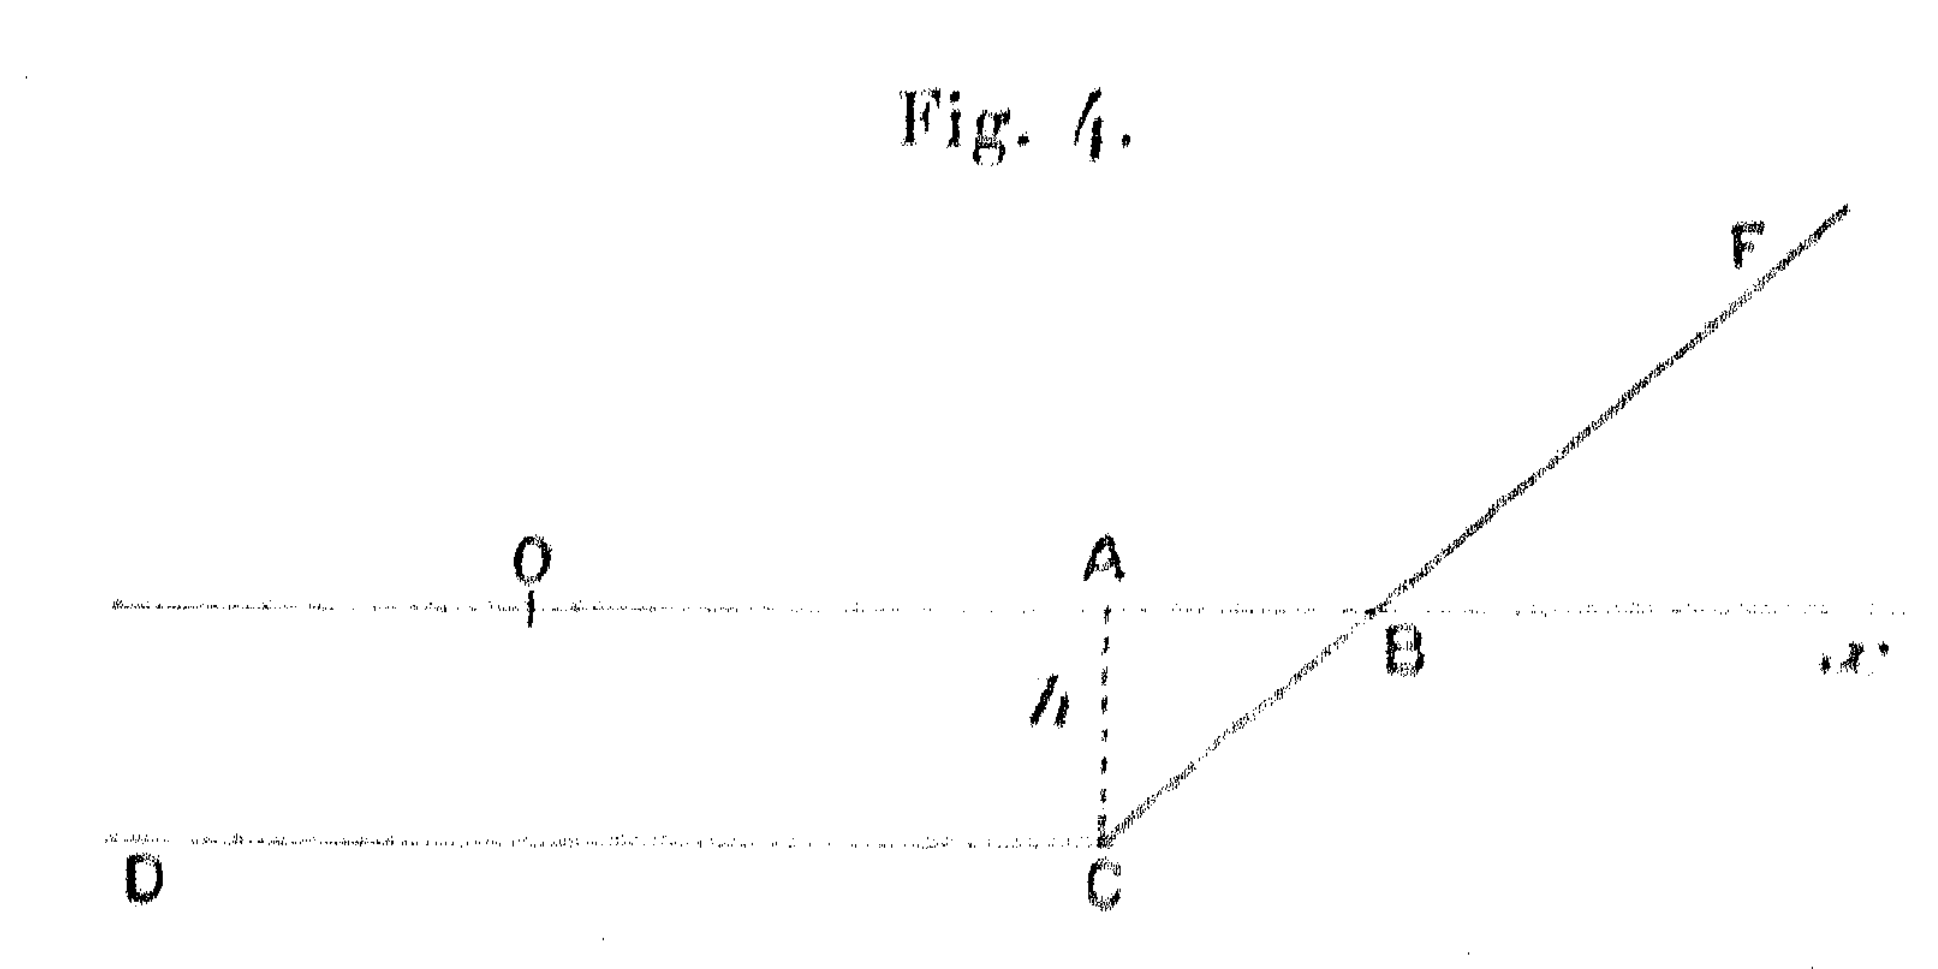
\includegraphics[width=0.6\textwidth]{fig4.png}
    Courbe de probabilité extraite de la thèse de Bachelier (p. 36), représentant la densité gaussienne des cours futurs à l’instant $t$.
\end{center}

\vspace{0.5cm}

\begin{center}
    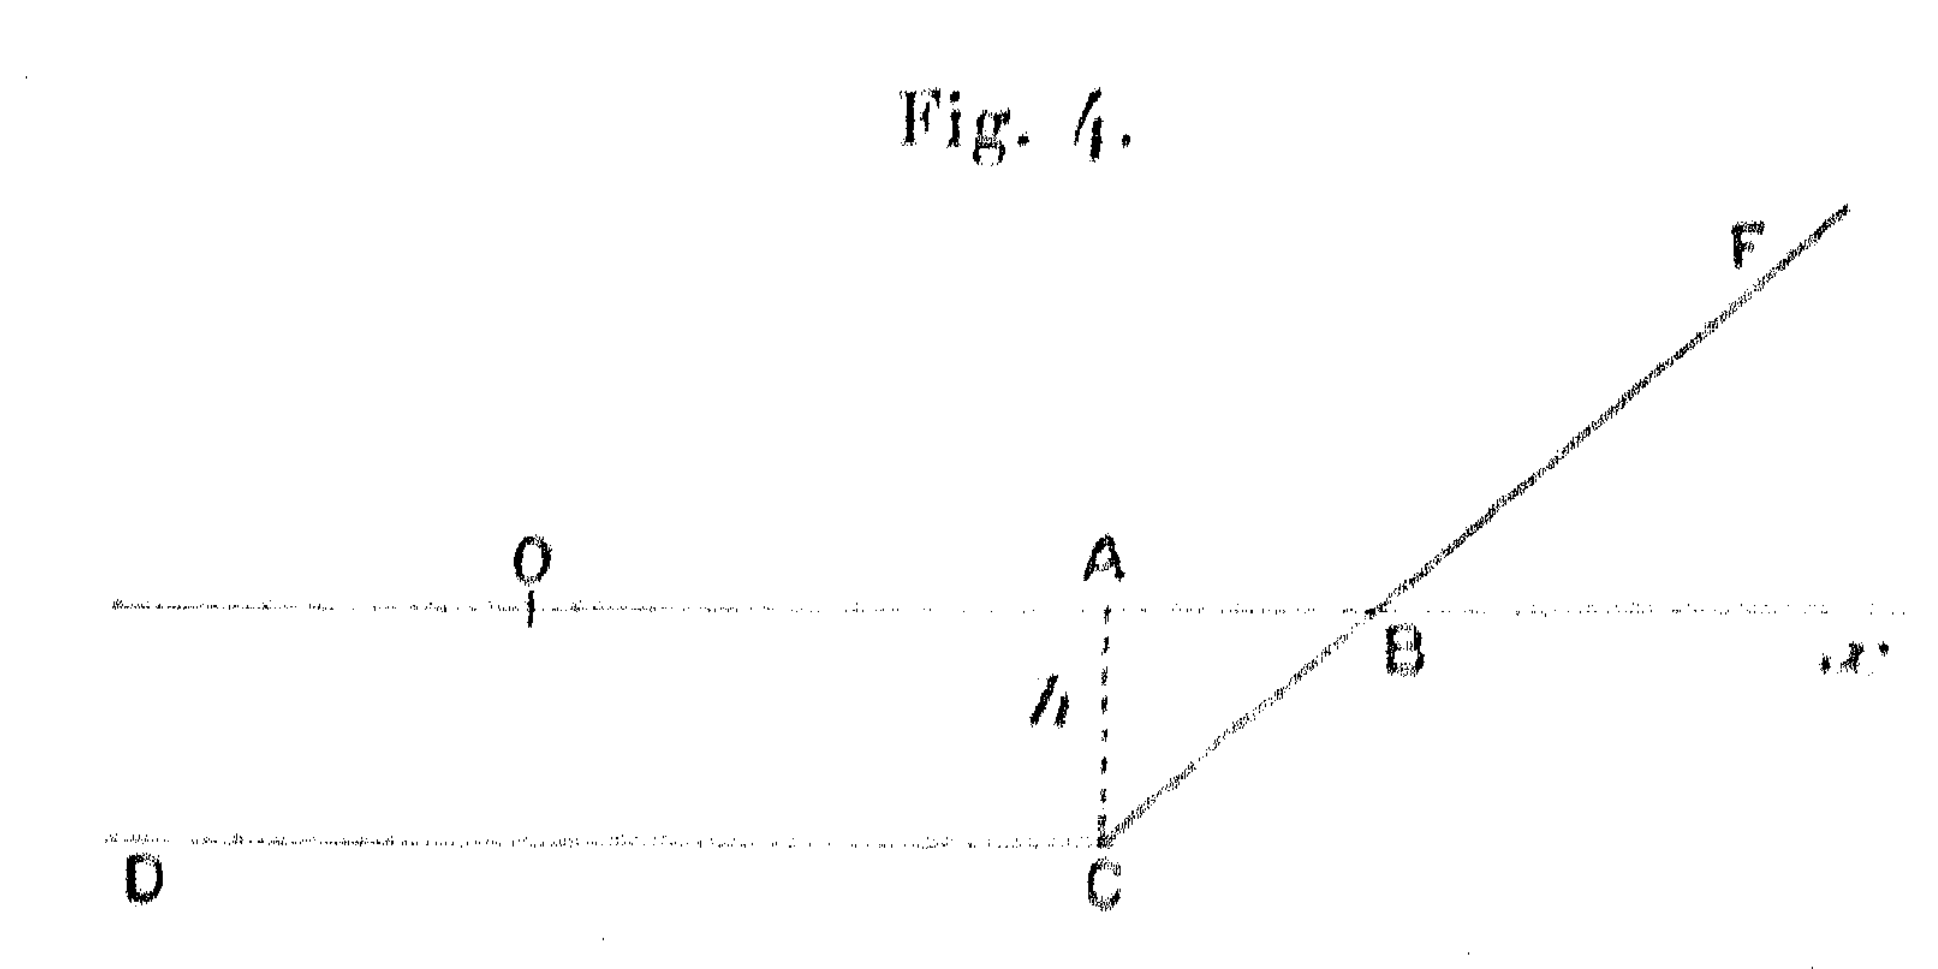
\includegraphics[width=0.65\textwidth]{fig4.png}
    Illustration de la valeur moyenne d’une prime simple selon l’écart du cours (p. 53).
\end{center}

\textit{Remarque} : Ces figures peuvent être recréées en Python/Matplotlib ou TikZ pour une meilleure qualité typographique.

\subsection*{B. Détails de formules mathématiques}

\textbf{1. Espérance positive d’une prime simple} :
\[
\mathbb{E}[(X - a)^+] = \int_a^{\infty} (x - a)\, p(x,t)\, dx
= \frac{\sigma\sqrt{t}}{\sqrt{2\pi}} \exp\left(-\frac{a^2}{2\sigma^2 t}\right) - a\left(1 - \Phi\left(\frac{a}{\sigma \sqrt{t}}\right)\right)
\]

\textbf{2. Probabilité de succès d’une prime} :
\[
\mathbb{P}(X > a) = \int_a^{\infty} p(x,t)\, dx = 1 - \Phi\left(\frac{a}{\sqrt{2t}}\right)
\]

\textbf{3. Solution fondamentale de l’équation de la chaleur} :
\[
p(x,t) = \frac{1}{\sqrt{4\pi t}} \exp\left(-\frac{x^2}{4t}\right)
\]

\textbf{4. Écart-type en fonction du temps} :
\[
\text{Var}(X_t) = 2t, \qquad \sigma(t) = \sqrt{2t}
\]

\subsection*{C. Références bibliographiques}

\begin{itemize}
    \item Bachelier, L. (1900). \textit{Théorie de la spéculation}. Annales scientifiques de l’École Normale Supérieure, 3\textsuperscript{e} série, 17, 21–86.

    \item Samuelson, P. A. (1955). \textit{Brownian Motion in the Stock Market}. Cowles Commission Discussion Paper.

    \item Black, F., \& Scholes, M. (1973). \textit{The Pricing of Options and Corporate Liabilities}. Journal of Political Economy, 81(3), 637–654.

    \item Fama, E. (1965). \textit{The Behavior of Stock Market Prices}. Journal of Business, 38(1), 34–105.

    \item Jarrow, R., \& Protter, P. (2004). \textit{A short history of stochastic integration and mathematical finance}. In: \textit{The Legacy of the Notion of Probability}, ed. by J.-P. Aubin.
\end{itemize}

\subsection*{D. Glossaire des termes techniques}

\begin{description}
    \item[Espérance mathématique :] Valeur moyenne d’une variable aléatoire, pondérée par sa probabilité.
    \item[Prime :] Prix payé pour acquérir une option ; aussi appelée « valeur de l’option ».
    \item[Cours vrai :] Valeur théorique du titre, centrée dans la loi de probabilité.
    \item[Processus de diffusion :] Modèle aléatoire continu dont l’évolution dépend d’une équation aux dérivées partielles.
    \item[Écart-type :] Racine carrée de la variance ; mesure de la dispersion autour de la moyenne.
    \item[Martingale :] Processus stochastique sans tendance, pour lequel l’espérance future est égale à la valeur actuelle.
    \item[Mouvement brownien :] Processus gaussien à accroissements indépendants et stationnaires, utilisé comme base des modèles de prix.
    \item[Option :] Contrat financier donnant le droit (mais non l’obligation) d’acheter ou de vendre un actif à un prix donné.
    \item[Diffusion additive vs. multiplicative :] Une diffusion additive implique une loi normale des prix ($S_t$), alors qu’une diffusion multiplicative implique une loi log-normale.
\end{description}

\end{document}